\phantomsection
\addcontentsline{toc}{section}{Lampiran A: Form Penggunaan Generative AI}
\section*{Lampiran A: Form Penggunaan \textit{Generative AI}}

\begingroup
\small
\begin{center}
  \textbf{FORMAT DEKLARASI PENGGUNAAN AI} \\
  \textbf{SURAT PERNYATAAN PENGGUNAAN AI}
\end{center}

Dengan ini, \sout{saya}/kami*:
\begin{center}
\begin{tabular}{lll}
  Nama/NIM & : & Stevanus Agustaf Wongso / 13524020, \\
   & & Jonathan Kris Wicaksono / 13524023, \\
   & & Made Branenda Jordhy / 13524026, \\
   & & Ray Owen Martin / 13524033, \\
   & & Philipp Hamara / 13524101 \\
  Fakultas/Sekolah & : & STEI ITB \\
  Kode Mata Kuliah & : & IF3170 \\
  Nama Mata Kuliah & : & Inteligensi Artifisial \\
  Judul Tugas/Proposal & : & Tugas Besar 2 (\textit{Supervised Learning}) \\
\end{tabular}
\end{center}

Menyatakan bahwa \sout{saya}/kami* menggunakan/\sout{tidak menggunakan}* AI dalam
pengerjaan maupun penyusunan luaran tugas pada mata kuliah yang tertulis
di atas.

Jika Ya, maka alat AI/kecerdasan buatan yang digunakan adalah: asisten AI
untuk diskusi konsep pemrograman.

\begin{center}
  \footnotesize
  \begin{tabular}{|>{\raggedright\arraybackslash}p{7cm}|c|c|}
    \hline
    \textbf{Lingkup Pekerjaan} & \textbf{Digunakan?} & \textbf{Tingkat Penggunaan} \\ \hline
    \textbf{Pemeriksaan Ejaan:} menggunakan tools seperti Grammarly,
    Paperpal, DeepL, Quillbot, Grammarbot, LanguageTool, ProWritingAid,
    ChatGPT, Google Gemini, atau sejenisnya. & Tidak & -- \\ \hline
    \textbf{Pembuatan Teks:} menggunakan tools seperti ChatGPT, Gemini,
    Paperpal, Copilot, GrammarlyGO, WordAI, WriteSonic, Jasper, Jenni AI,
    atau sejenisnya. & Tidak & -- \\ \hline
    \textbf{Bantuan Diskusi dalam Penyusunan Konten:} menggunakan tools
    seperti ChatGPT, Gemini, Copilot, Perplexity, Jenni AI,
    Zoom-Companion, atau sejenisnya. & Ya & Kecil \\ \hline
    \textbf{Pembuatan Gambar, Video, dan/atau Grafik:} menggunakan tools
    seperti Craiyon, DALL-E, Midjourney, Stable Diffusion, Microsoft
    Designer, Gemini, Canva AI, atau sejenisnya. & Tidak & -- \\ \hline
    \textbf{Lainnya, Jelaskan:} & -- & -- \\ \hline
  \end{tabular}
\end{center}

\sout{Saya}/Kami* juga menyatakan bahwa setiap penggunaan AI/kecerdasan buatan
yang dilakukan pada mata kuliah tersebut telah dinyatakan di dalam surat
ini.

\smallskip
\noindent Bandung, 24 November 2026

\smallskip
\begin{center}
  \footnotesize
  \begin{tabular}{ccc}
    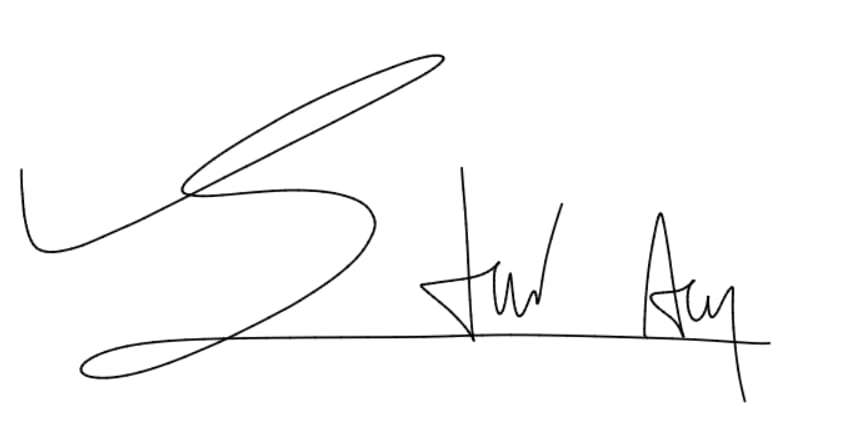
\includegraphics[height=1.35cm, keepaspectratio]{assets/ttd/ttd_stevanus.png} & \hspace{1.8cm} &
    
\includegraphics[height=1.35cm, keepaspectratio]{assets/ttd/ttd_jonathan.png} \\
    (Stevanus Agustaf Wongso) & & (Jonathan Kris Wicaksono) \\
    NIM 13524020 & & NIM 13524023 \\[0.25cm]
    
\includegraphics[height=1.35cm, keepaspectratio]{assets/ttd/ttd_jordhy.jpeg} & &
    
\includegraphics[height=1.35cm, keepaspectratio]{assets/ttd/ttd_owen.jpeg} \\
    (Made Branenda Jordhy) & & (Ray Owen Martin) \\
    NIM 13524026 & & NIM 13524033 \\[0.25cm]
    \multicolumn{3}{c}{
\includegraphics[height=1.35cm, keepaspectratio]{assets/ttd/ttd_philipp.jpeg}} \\
    \multicolumn{3}{c}{(Philipp Hamara)} \\
    \multicolumn{3}{c}{NIM 13524101} \\
  \end{tabular}
\end{center}
\endgroup
